\chapter{Evaluation}

\section{Fragebögen}
Die Versuchspersonen wurden jeweils vor und nach dem Experiment gebeten, einen Fragebogen auszufüllen. Der erste Fragebogen vor dem Experiment beinhaltet Fragen zur Person selbst, der zweite Fragebogen nach dem Experiment beinhaltet Fragen zu den Eindrücken der Person während des Experiments. Beide Fragebögen lagen ausschließlich auf Deutsch und in digitaler Form vor. Die Fragen des zweiten Fragebogens wurden zur Hilfe der Verständlichkeit aus dem Englischen ins Deutsche übersetzt. Zur Erstellung der Fragebögen wurde das Online Tool Google Forms verwendet, welches die gewünschte Funktion einer Likert-Skala sowie das Exportieren der Daten als Microsoft Excel Datei unterstützt. Die kompletten Fragebögen befinden sich im Anhang.
Der erste Fragebogen mit dem Namen \textit{Demographische Fragen} enthielt zu beginn eine schriftliche Beschreibung des Versuchs, was die Person erwartet und wie lange der Versuchs ungefähr dauern wird sowie ein Bild, welches die Sicht des Benutzers in der Anwendung zeigt. Nachdem der Proband zur Teilnahme am Versuch zugestimmt hat, musste die vor der Teilnahme zugewiesene Teilnehmer ID eingetragen werden. Die ID sollte dabei helfen, die Antworten der beiden Fragebögen einander zuzuordnen. Zunächst wurden die Personen nach Geschlecht und Alter gefragt. Die nächste Frage beschäftigt sich damit, ob die Testpersonen eine Sehhilfe benötigen oder eine Farbsehstörung aufweisen. Die letzte Frage des ersten Fragebogens bezieht sich auf die Vorkenntnisse der Person im Bezug auf Virtuelle Realität (VR). 
Im zweiten Fragebogen, der nach dem Experiment vorgelegt wurde, sollte als erstes die erreichte Punktzahl sowie die einzelnen Plus- und Minuspunkte während des Versuchs eingetragen werden. Als nächstes wurde gefragt, ob die Person Übelkeit während des Experiments verspürt hatte.
Im Anschluss wurden die Fragen eines Fragebogens für Avatar Embodiment in VR (VR-AEB) von Gonzalez-Franco und Peck \cite{Gonzalez-Franco2018} gestellt. Bei dem Fragebogen handelt es sich um einen Vorschlag für einen Standard Fragebogen für Embodiment, da noch kein solcher standardisierter Fragebogen um Embodiment für Avatare zu messen, existiert. Gonzalez-Franco und Peck analysierten dabei über 30 Experimente, die im Zeitraum von 1998 bis 2018 stattfanden und sich mit Embodiment auseinandersetzten. Die in diesen Experimenten gestellten Fragen wurden klassifiziert, wobei sechs Kategorien an Fragen enstanden.
Die Reihenfolge der gestellten Fragen wurde, wie in Gonzalez-Francos und Pecks Paper vorgeschlagen, Randomisiert. Jede der Fragen konnte auf einer sieben Punkte Likert-Skala von -3 (Ich stimme überhaupt nicht zu) über 0 (Neutral), bis zu +3 (Ich stimmte voll und ganz zu) beantwortet werden.
Von den 25 Fragen des AEQ wurden 16 in den Finalen Fragebogen aufgenommen, da einige der Fragen nicht auf das Experiment zutreffend waren. Fragen, die sich mit Berührung auseinandersetzen sowie die komplette Kategorie \textit{Reaktion auf externe Stimuli} wurden daher nicht gefragt.
Nach dem Fragebogen zu Embodiment, wurde die Person Fragen aus dem NASA Task Load Index \cite{HART1988} gefragt. Dabei soll die wahrgenommene Belastung im Hinblick auf die Aufgabe gemessen werden.
Zuletzt wurde der Testperson die Möglichkeit gegeben, in einem freien Kommentarfeld zusätzliche Eindrücke und Kommentare zu dem Experiment zu geben.

Zusätzlich zu den Fragebögen wurde eine Liste geführt, welche Teilnehmer ID die zusätzlichen Tracker verwendet hat und welche nicht. Innerhalb dieser Liste wurden zusätzliche Kommentare der Teilnehmer erfasst, die sie während des Experiments gesagt wurden.


\section{Auswertung}
Die statistische Auswertung der Daten wurde in IBM SPSS Statistics ausgeführt. 
Da die Richtigkeit der Hypothesen nicht mathematisch bewiesen werden kann, wird zu jeder Hypothese eine Nullhypothese formuliert, die das Gegenteil aussagt. Es kann die Wahscheinlichkeit errechnet werden, mit der die Nullhypothese abgelehnt wird, wodurch sich Schlüsse auf die Richtigkeit der Hypothese ziehen lassen. Die jeweils zu untersuchende Hypothese H1 wird Alternativhypothese genannt. Im folgenden werden alle drei aufgestellten Alternativhypothesen mit ihrer jeweiligen Nullhypothese gelistet.

\begin{itemize} 

\item \textbf{H1 Embodiment:} Der Grad an Kontrolle über einen Avatar hat Auswirkungen auf das Embodiment.
\item \textbf{H0 Embodiment:} Der Grad an Kontrolle über einen Avatar hat keine Auswirkungen auf das Embodiment.

\item \textbf{H1 Workload:} Der Grad an Kontrolle über einen Avatar hat Auswirkungen auf den gefühlten Grad an Belastung hinsichtlich der Aufgabe.
\item \textbf{H0 Workload:} Der Grad an Kontrolle über einen Avatar hat keine Auswirkungen auf den gefühlten Grad an Belastung hinsichtlich der Aufgabe.

\item \textbf{H1 Punktzahl:} Der Grad an Kontrolle über einen Avatar hat Auswirkungen auf den Erfolg in einer Bewegungsorientierten Aufgabe.
\item \textbf{H0 Punktzahl:} Der Grad an Kontrolle über einen Avatar hat keine Auswirkungen auf den Erfolg in einer Bewegungsorientierten Aufgabe.

\end{itemize}

Der p-Wert, der die Wahrscheinlichkeit angibt, mit der die Nullhypothese fälschlicherweise verworfen wird, ist als 0,05 festgelegt.
Liegt die errechnete Wahrscheinlichkeit unter dem p-Wert von 0,05 kann angenommen werden, dass das Ergebnis nicht zufällig entstanden ist. Liegt die errechnete Wahrscheinlichkeit unter einem p-Wert von 0,10 kann zumindest ein Trend angenommen werden.
Die Wahrscheinlichkeit wird berechnet, indem angenommen wird, dass die Nullhypothese H0 wahr ist. Wenn sich herausstellt, dass die Nullhypothese trotz der unterschiedlicher Versuchbedingungen wahr ist, kann angenommen werden dass die Versuchsbedungungen keinen Einfluss auf die zu untersuchenden Effekte hat. Das Ziel ist es somit, die Nullhypothese zu widerlegen.
Die Berechnung der Nullhypothese erfolgt individuell für jede der Fragen in den Fragebögen.

Damit die Statistische Auswertung über einen zweiseitigen t-Test möglich ist, müssen die Ergebnisse der Experiments auf die Normalverteilung überprüft werden. Nur wenn die Ergebnisse normalverteilt sind, kann der t-Test durchgeführt werden. Der zweiseitige t-Test wird für Experimente verwendet, die zwei Gruppen mit den selben Fragen aufweisen und rechnet mit Mittelwerten. Für die Ergebnisse, die nicht normalverteilt sind, wird der Mann-Whitney U-Test durchgeführt. Der Mann-Whitney U-Test ist eine Version des t-Tests, der auf nicht normalverteilte Daten angewendet werden kann. Die Daten müssen dafür jedoch in Ränge eingestuft sein. Der dabei errechnete Z-Wert gibt an, ob die Wahrscheinlichkeit der Nullhypothese unter den festgelegten 5 Prozent ist. Dafür existieren Tabellen, in denen der Z-Wert nachgeschaut werden kann?????? Die Z-Verteilung mit Tabelle kann nur eingesetzt werden, wenn die Anzahl der Probanden größer als 20 ist, was im durchgeführten Experiment mit 21 Probanden der Fall war.


\section{Avatar Embodiment Questionnaire}
Der im Experiment verwendetet Vorschlag für einen standardisierten Avatar Embodiment Fragebogen von Gonzalez-Franco und Peck im Jahr 2018 \cite{Gonzalez-Franco2018} mit dem Namen Avatar Embodiment Questionnaire (AEQ) besteht aus 25 Fragen, die in folgende Kategorien unterteilt sind:
\begin{enumerate} 

\item \textbf{Body Ownership (Körper Zugehörigkeit)}\\
Beschreibt die Zughörigkeit der Person zu dem sichtbaren, virtuellen Körpers unabhängig von dem Standort des virtuellen Körpers. Diese Kategorie an Fragen wurde in 96 Prozent der von Gonzalez-Franco und Peck analysierten Fragebögen verwendet. \cite{Gonzalez-Franco2018}. Fragen aus der Kategorie Body Ownership beschäftigen sich damit, ob sich eine Person unabhängig des Kontexts mit einem virtuellen Körper identifizieren kann.

\item\textbf{Agency and Motor Control (Entscheidungsfreiheit, Motorische Kontrolle über den Körper)}\\
Misst den Grad an Kontrolle des Benutzers über den virtuellen Körper und dessen Gliedmaßen. Die Fragen aus dieser Kategorie sind besonders Interessant für dieses Experiment, da der einzige Unterschied zwischen den beiden Bedingungen der Grad an Bewegungsmöglichkeiten ist. Die Fragen beschäftigen sich damit, ob der Körper sich so bewegt wie der Benutzer sich in Wirklichkeit bewegt.

\item\textbf{Tactile sensations (Haptische Stimulation)}\\
Misst, ob Berührungen oder Kollisionen des Avatars mit der Umgebung sich auf die Person auswirken. Aus dieser Kategorie wurden zwei von vier Fragen verwendet, da sich zwei der Fragen zu stark mit expliziten Berührungen auseinandersetzen, die nicht im Versuchsaufbau vorkommen.

\item\textbf{Location of the body (Standort des Körpers)}\\
Zwei der drei Fragen über den Standort des Körpers wurden gefragt. Die beiden Fragen handeln von dem Bezug des Standorts des realen Körpers zum Standort des virtuellen Körpers. Die dritte Frage wird in Gonzalez-Francos und Pecks Paper explizit als optional markiert und soll nur gefragt werden, wenn sich der virtuelle Körper nicht dort befinden soll, wo sich der reale Körper befindet.

\item\textbf{Appearance (Äußere Erscheinung)}\\
Über die Äußere Erscheinung wurden die Probanden drei der vier vorgeschlagenen Fragen gefragt. In den Fragen kommt vor, wie sich die Person äußerlich mit dem Avatar identifizieren kann. Frage 20 wurde nicht in den Fragebogen aufgenommen, da darin die Kleidung des Avatars eine Rolle spielt, der Avatar in der Anwendung jedoch als Holzpuppe ohne Kleidung dargestellt wird.

\item\textbf{Response to external stimuli (Reaktion auf externe Stimulation)}\\
Diese Kategorie wurde nicht in den Fragebogen aufgenommen, da sich die Fragen darin mit einer expliziten Angst oder Gefahr, in der sich der virtuelle Körper befindet, beschäftigt und dies nicht in dem Versuch vorkommt.

\end{enumerate}

Durch Addition der angegebenen Werte der Fragen innerhalb der Kategorien kann ein Wert für jede Kategorie pro Person bestimmt werden. Dabei erhalten Fragen, die nach dem Stand der Forschung ein Indikator für Embodiment sind, ein positives Vorzeichen. Ist eine Frage des Fragebogens ein Indikator gegen Embodiment, erhält die Frage in der Rechnung ein Negatives Vorzeichen.
Manche Fragen bilden innerhalb der Kategorien Paare, wobei die Fragen die Negation zu sich gegenseitig bilden.

Die Kategorien können wiederum zu einem gesamten Embodiment Wert zusammengefasst werden. Die Werte der Kategorien werden aufsummiert, jede Kategorie wird zusätzlich mit einem Multiplikator versehen, der die Wichtigkeit der Kategorien im Hinblick auf Embodiment  zueinander repräsentiert. Im folgenden die verwendete Formel ohne die Kategorie \textit{Response}:\\
Total Embodiment = ((Ownership/5) * 2 + (Agency/4) * 2 + Tactile Sensation/4 + (Location/3) * 2 + Appearance/4) / 9




\subsection{Avatar Embodiment Questionnaire Ergebnisse}
Die Daten aus dem VR-Avatar Embodiment Fragebogen liefern keine statistisch signifikanten Ergebnisse. Keiner der Werte liegt innerhalb der festgelegten Signifikanz 0,10 (p<0,10) um überhaupt einen Trend anzuzeigen. Dennoch weisen manche Fragen eine Gemeinsamkeit der Antworten zwischen den beiden Gruppen vor und wenige der Fragen liegen nur knapp über einem p-Wert von 0,10. Alle Beobachtungen müssen dennoch unter der Annahme betrachtet werden, dass die Ergebnisse nur zufällig aufgrund der geringen Gruppengröße von 21 Teilnehmern entstanden sind.

\begin{figure}[h]
  \makebox[\textwidth]{
    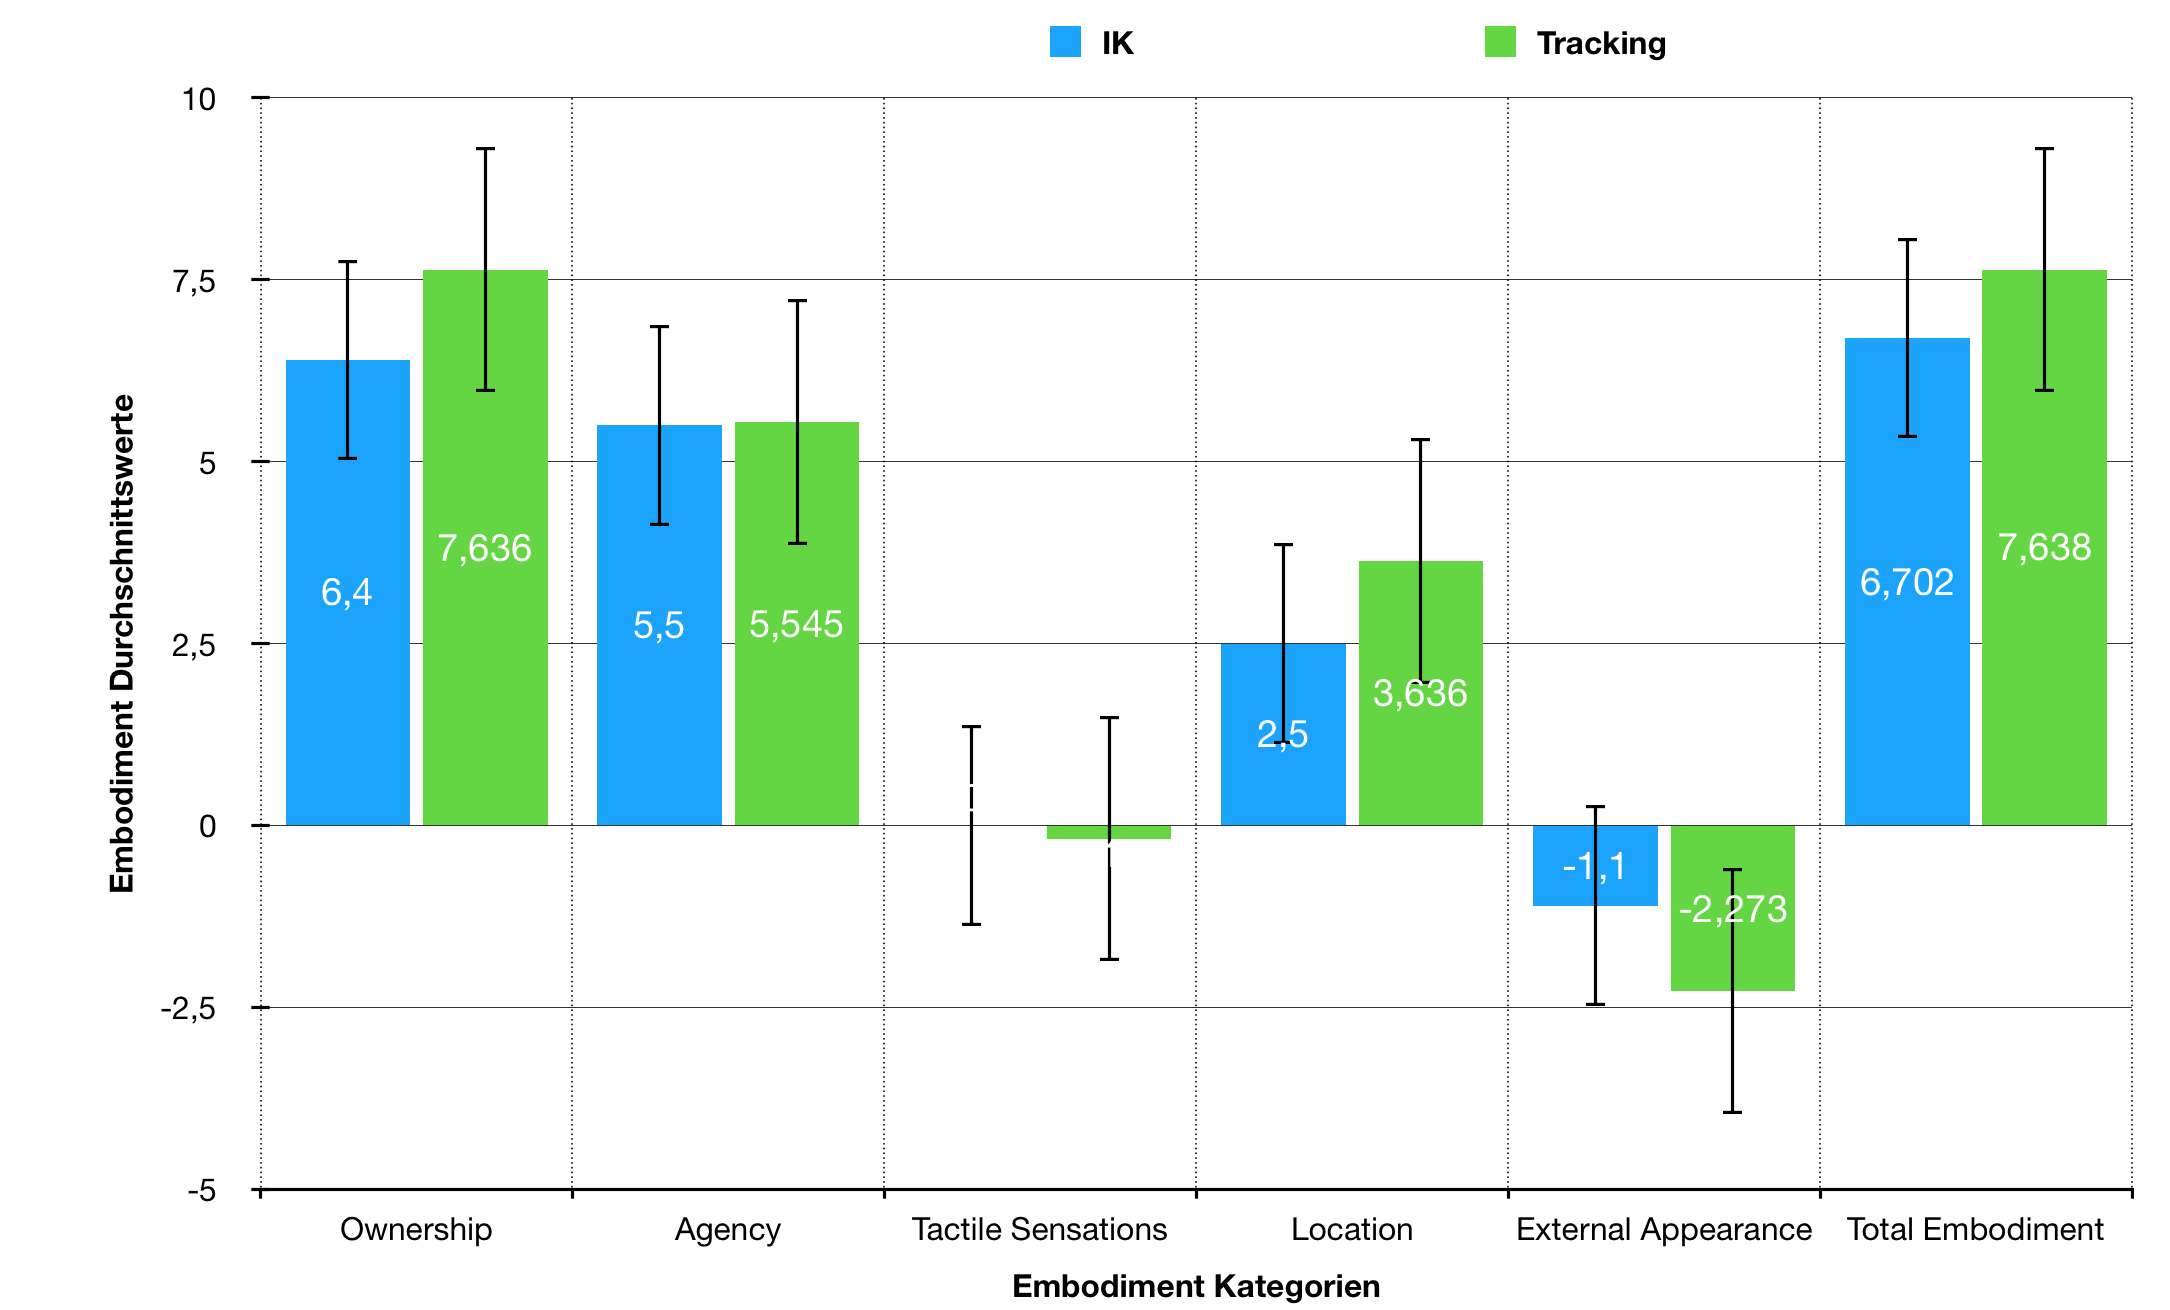
\includegraphics[width=\textwidth]{Bilder/Diagramme/TotalEmbodiment-Kategorien.png}
  }
  \caption[Avatar Embodiment Durchschnitte pro Kategorie]{Vergleich der Gruppen pro Kategorie des Avatar Embodiment Fragebogens}
  \label{fig:TotalEmbodiment-Kategorien}
\end{figure}

Der Vergleich, wie die beiden Gruppen jeweils die Fragen der einzelnen Kategorien des Embodiment Fragebogens beantworteten, ist in Abbildung \ref{fig:TotalEmbodiment-Kategorien} dargestellt. Dabei repräsentieren die blauen Balken die Gruppe ohne zusätzliche Tracker dar, die grünen Balken die Gruppe mit den zusätzlichen Trackern. Die erstem fünf Balkenpaare bilden jeweils eine der fünf Kategorien aus denen die Fragen stammen. Das letzte Balkenpaar zeigt den gesamten mittleren Embodiment Wert pro Gruppe dar. Die Fehlerbalken beschreiben einen Standardfehler.
Zwar ist der Wert des gesamten Embodiments in der Bedingungen mit zusätzlichen Trackern höher als der Wert der anderen Bedingung, da die Ergebnisse jedoch nicht statistisch signifikant sind und die Standardfehler größer sind, als der Unterschied zwischen den beiden Gruppen, können daraus keine Schlüsse gezogen werden. Auffällig ist, dass die Kategorie Agency fast keinen Unterschied der Gruppen mit Werten von 5,5 und 5,545 aufweist, obwohl der Versuch so konzipiert ist, dass die Agency der einzige Unterschied zwischen den beiden Versuchsbedingungen darstellen sollte. Auch hieraus lassen aufgrund der niedrigen statistischen Signifikanz sich keine Schlüsse ziehen, ebenso in allen anderen Kategorien.

Abbildung \ref{fig:OwnershipScores} zeigt die Durchschnittlichen Werte der Antworten für jede Frage der Kategorie 1.: Ownership. Die Formel für das Gesamtergebnis der Kategorie Ownership lautet: Ownership = (Q1 - Q2) - Q3 + (Q4 - Q5)
 .Dabei bilden jeweils die Fragen Q1 und Q2 sowie Q3 und Q4 ein Paar, bei dem jeweils die erste Frage das Gegenteil der zweiten Frage bildet. Die Fragen mit positiven Vorzeichen Q1 und Q4 sind Indikatoren für Body Ownership. Die Probanden beider Versuchsbedingungen konnten sich bedingt mit dem Avatar identifizieren, was man an den neutralen Werten der Fragen Q1 und Q4 zwischen null und eins erkennen kann. Der Grund dafür liegt vermutlich in der Abstrakten Form des eingesetzten Avatars, der zwar Menschliche Proportionen besitzt, jedoch keine Details wie Kleidung, Haare oder ein Gesicht.
Die jeweilige andere Frage der Paare Q2 und Q5 sowie die alleinstehende Frage Q3, die alle negative Vorzeichen aufweisen, also Indikatoren gegen Ownership und Embodiment sind, befinden sich dafür alle im Negativen Bereich zwischen -1 und -3. Diese drei Fragen beschäftigen sich damit, ob der Avatar ein zusätzlicher Körper oder der Körper einer anderen Person darstellt. Damit fühlten sich die Probanden zwar nicht mit dem Avatar-Körper verbunden, schließen jedoch aus, dass der Körper nicht ihre virtuelle Repräsentation darstellt.
Die beiden Versuchsbedingen weisen bei keiner der fünf Ownership-Fragen signifikanten Unterschiede bei den Antworten auf, womit vermutet werden kann, dass die Bedingungen keinen Einfluss auf Body-Ownerhsip haben. Diese Beobachtung stimmt mit früheren Veröffentlichten Untersuchungen überein, bei denen unter anderem der Zusammenhang zwischen Agency und Ownership untersucht wurde\cite{Koilias2019}\cite{Kalckert2012}.

\begin{figure}[h]
  \makebox[\textwidth]{
    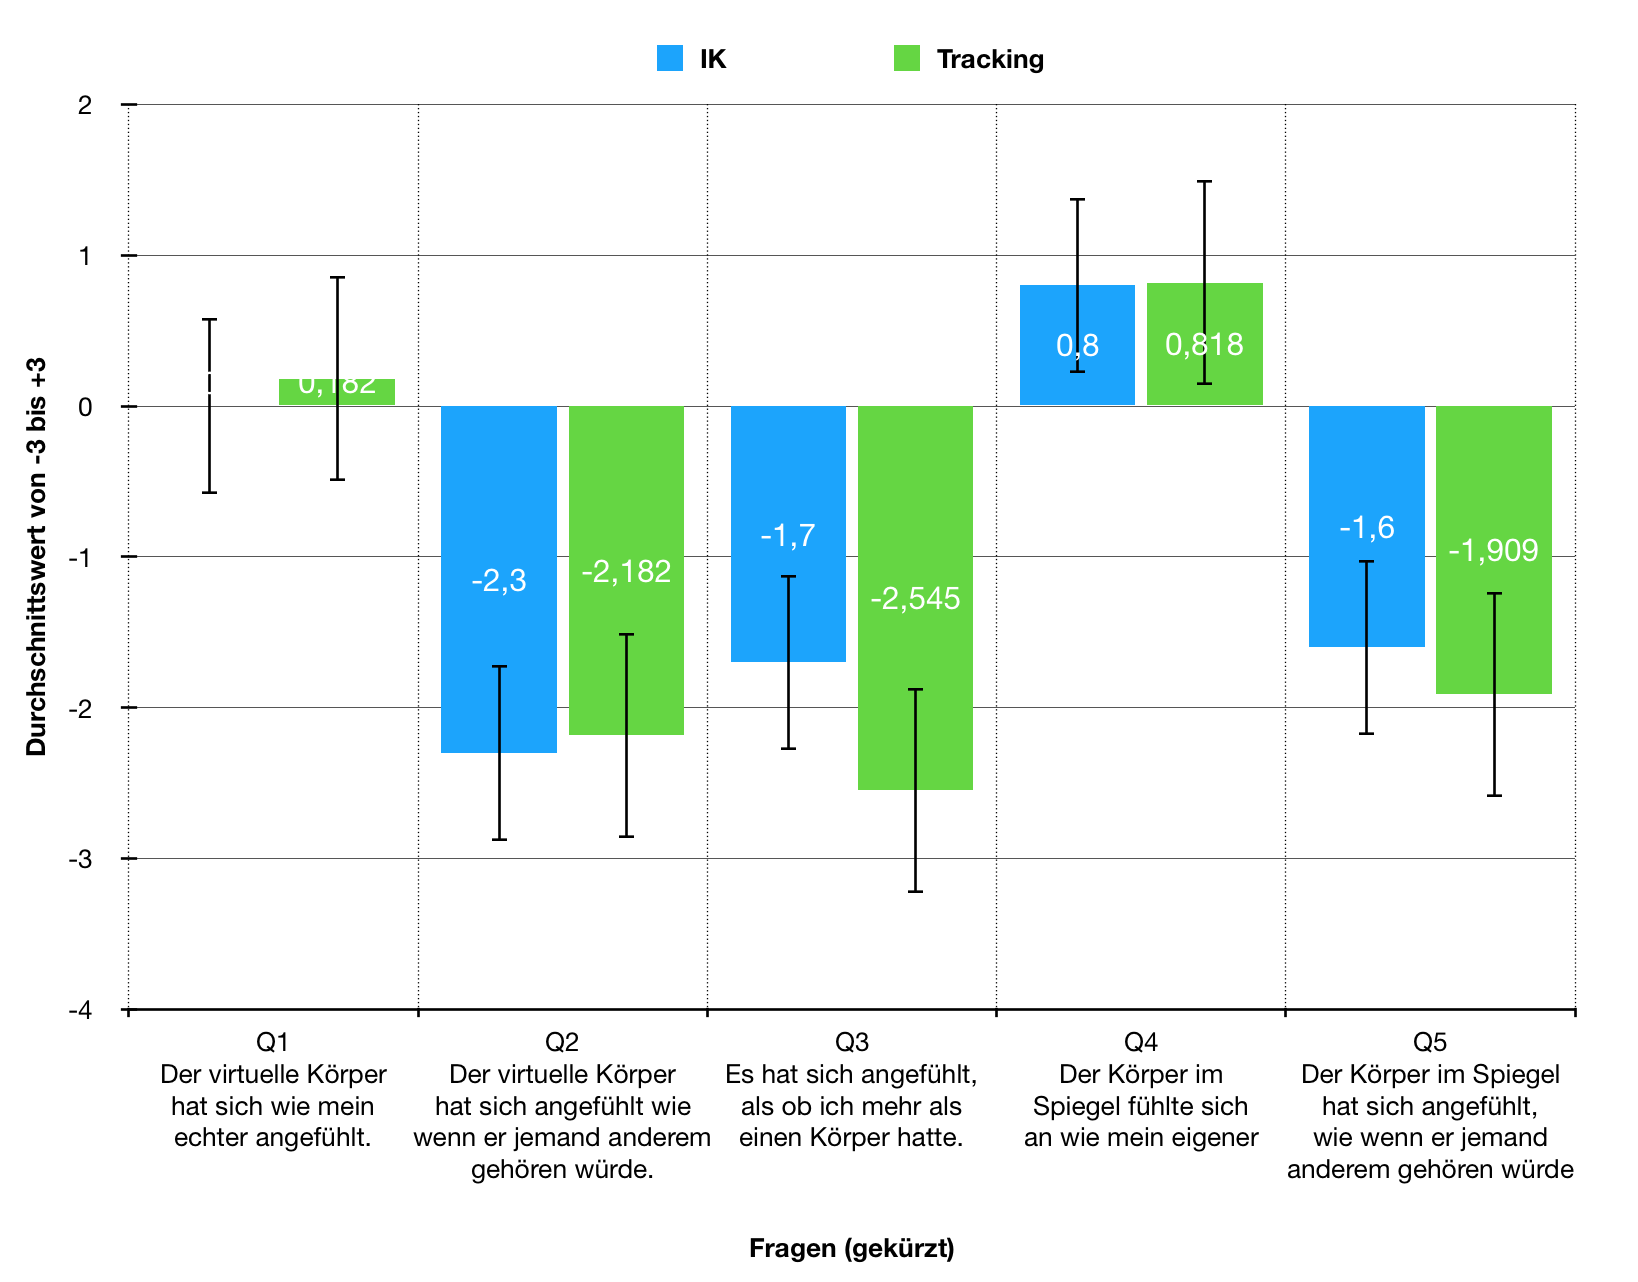
\includegraphics[width=\textwidth]{Bilder/Diagramme/OwnershipScores.png}
  }
  \caption[Durchschnittlicher Wert der Antworten in der Kategory Ownership]{Durchschnittlicher Wert der Antworten in der Kategory Ownership}
  \label{fig:OwnershipScores}
\end{figure}



In Abbildung \ref{fig:AgencyScores} in die Antworten der Probanden der Kategorie Agency zu sehen. Der p-Wert von Frage Q7 beträgt 0,115 und ist somit nicht statistisch signifikant, liegt jedoch nur knapp über dem festgelegten Wert von p = 0,10 um einen Trend anzuzeigen. Die Restlichen Fragen in der Kategorie Angency liegen weit über dem p-Wert von 0,10, wodurch sich keine Aussagen über sie treffen lässt.

\begin{figure}[h]
  \makebox[\textwidth]{
    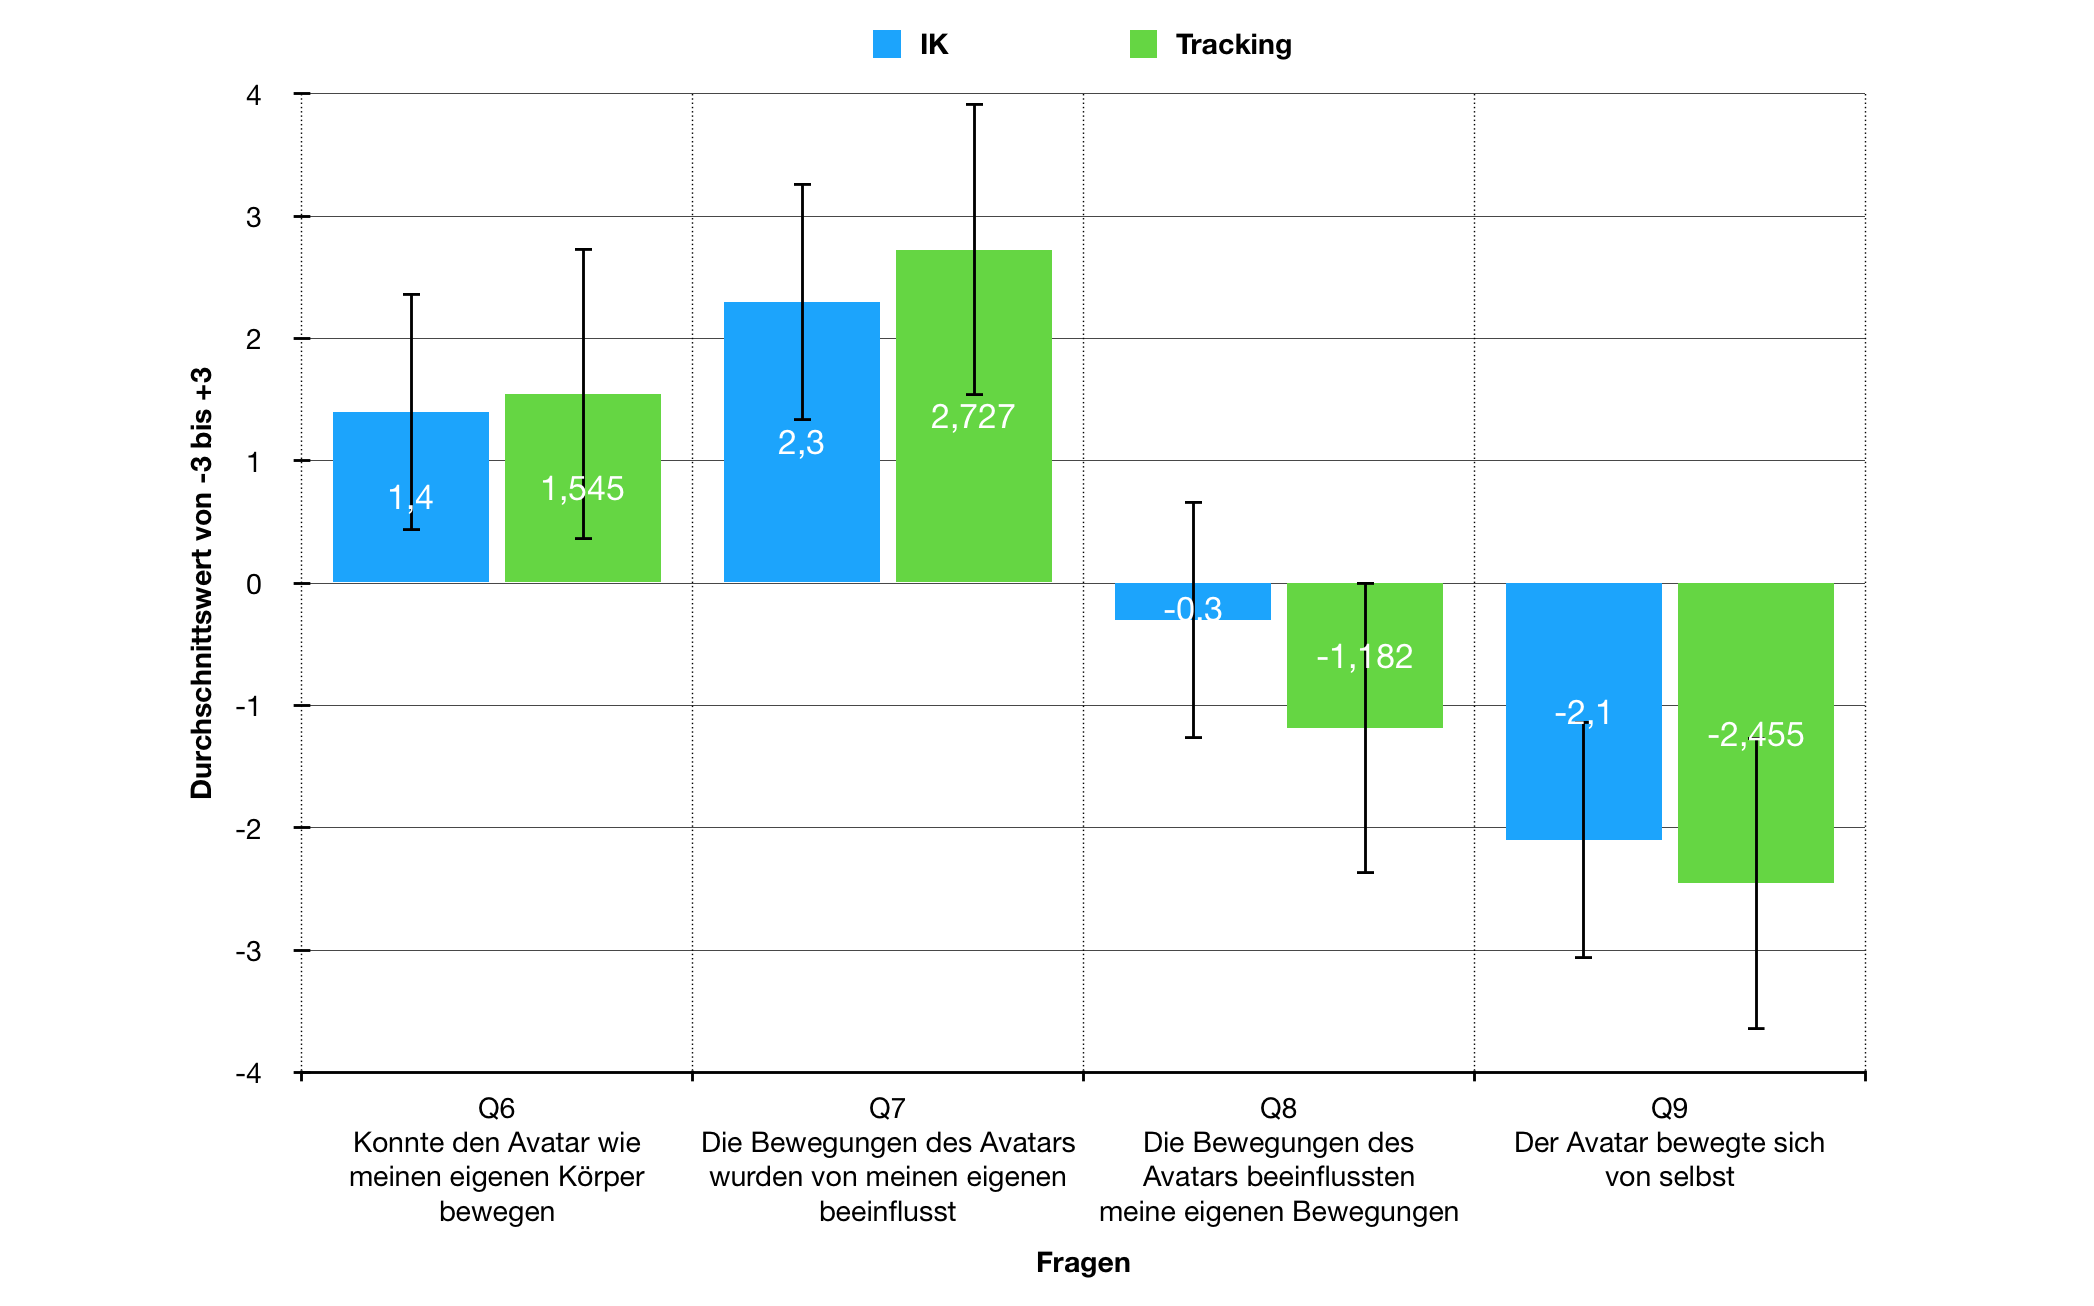
\includegraphics[width=\textwidth]{Bilder/Diagramme/Embodiment-Agency-Fragen.png}
  }
  \caption[Durchschnittlicher Wert der Antworten in der Kategory Agency]{Durchschnittlicher Wert der Antworten in der Kategory Agency}
  \label{fig:AgencyScores}
\end{figure}


Auch wenn nach Abtahi \cite{Abtahi2019} die Agency eine wichtige Rolle für das Embodiment in VR Anwendungen spielt, rückt die Agency je nach Kontext weit in den Hintergrund. Bereits ein einfacher Spaziergang in der Virtuellen Umgebung (VU) kann dafür sorgen, dass die Agency im Bezug auf das Embodiment eine merklich kleinere Rolle spielt. Da die Probanden während des Ausweichspiels trotz Spiegel keine Möglichkeiten hatten, sich in Ruhe den Avatar anzuschauen und auf die Bewegungen zu achten, kann vermutet werden, dass der Grad an Kontrolle über den Avatar keine nachweisbaren Auswirkungen auf das Embodiment hat. Diese Aussage deckt sich mit mehreren mündlichen Kommentaren der Probanden. Es wurde berichtet, dass das Ausweichspiel so viel Fokus erforderte, dass die Bewegungen des Avatar nicht auffielen besonders auffielen, selbst wenn durch verrutschen eines Trackers der Avatar unnatürliche Bewegungen aufwies.
Selbst Probanden die kommentierten, dass sich der Körper verzögert oder unnatürlich bewegt, bewerteten die Agency mit Punkten zwischen eins und drei. Ein Grund dafür könnte das Inter-Subjekt Versuchsdesign sein, da die Probanden keine Vergleichsmöglichkeiten der beiden Versuchsbedingungen hatten. Ein weiterer Grund wäre der Effekt, dass die Agency während einer Aufgabe eine merklich kleinere Rolle auf das Embodiment hat, als angenommen wurde.


\section{NASA TLX}


\section{Performanz der Benutzer}
Die unterschiedlichen Versuchsbedingungen hatten keinen Nachweislichen Einfluss auf die Erreichte Punktzahl der Benutzer. Die durchschnittlich erreichte Punktzahl der Gruppe ohne zusätzliche Tracker beträgt 21,6 Punkte, die der Gruppe mit zusätzlichen Trackern 22,9 Punkte. Die Daten sind dabei nicht statistisch signifikant, da der p-Wert 0,546 beträgt und somit weit über den festgelegten 0,05 liegt. Dieses Ergebnis ist nicht überraschend, da die Kontrolle über die Ellbogen und Knie des Avatars keine Vorteile beim Ausweichen der Hindernisse bringen. Lediglich die direkte Kontrolle der Füße könnte beim Ausweichen helfen, was aber nur in wenigen Fällen vorkommt.















